\begin{figure}[htbp]\centering
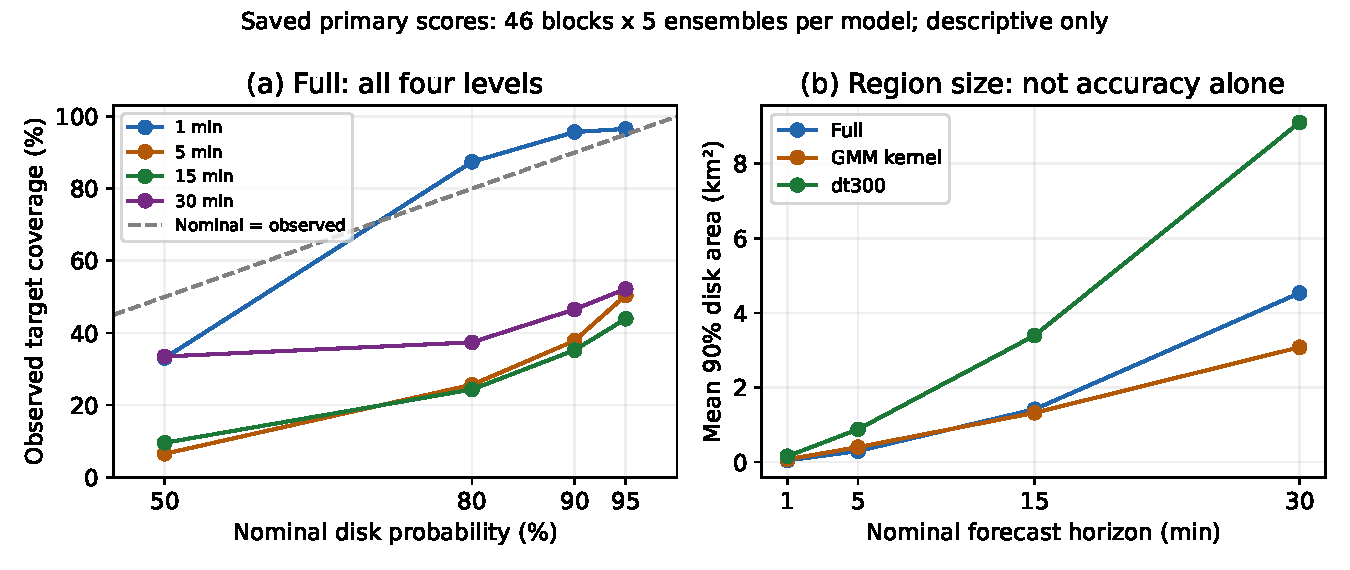
\includegraphics[width=\linewidth]{../figures/preliminary-calibration-area.pdf}
\caption{Calibration and size from the saved 46-block, five-seed summaries.
Left: 16 Full coverage values (four probability levels at four horizons);
closeness to the diagonal, not the highest curve, is the target. Right:
12 mean areas (three configurations at four horizons), to be read with
coverage rather than ranked alone. Connecting lines guide reading; they
do not add intermediate horizons or a calibration test.}
\label{fig:reader-calibration}\end{figure}
\begin{table}[htbp]\centering
\caption{Thirty-minute nominal 90\% disks: three configurations and nine
saved summary values. Each configuration uses 46 blocks and five ensembles
per block. Radius and area are averaged separately; the radius of the
mean area is not the mean radius.}\label{tab:reader-regions}
\begin{tabular}{lrrr}\toprule
Model & Coverage (\%) & Mean area (km$^2$) & Mean radius (m)\\\midrule
Full01 & 46.52 & 4.534 & 1183.6\\
GMM & 45.22 & 3.079 & 989.5\\
dt300 & 64.35 & 9.109 & 1692.8\\\bottomrule
\end{tabular}\end{table}
The dt300 disk is about twice Full's mean area, yet its inclusion rate
remains below the nominal 90\%. A larger region can include more targets
while its centre is less accurate. Conversely, GMM's smaller region does
not by itself establish better uncertainty prediction. Coverage averages
the same real target across five simulated disks in each block; there are
46 targets per horizon, not 230 independent targets. At block level this
five-seed inclusion proportion takes only 0, 20, 40, 60, 80 or 100\%.
The 552 points in the supplementary block plot can overlap at those six
levels; neither a block median of 100\% nor a dense-looking cluster is a
conditional calibration certificate. These observations support reporting
size and inclusion together while retaining the complete block summaries.
\FloatBarrier
